\section{Phần 1: Lý Thuyết Data Fitting và Minh Họa}

% ----------------------------------------------------------
\subsection{Bài Toán Data Fitting}

\subsubsection{Phát biểu bài toán tổng quát}

Cho tập dữ liệu $\mathcal{D} = \{(\mathbf{x}_i, y_i)\}_{i=1}^{n}$ với
$\mathbf{x}_i \in \mathbb{R}^p$, $y_i \in \mathbb{R}$.
Mô hình hồi quy tuyến tính giả thiết quan hệ:
\begin{equation}
    y_i = \beta_0 + \beta_1 x_{i1} + \beta_2 x_{i2} + \cdots + \beta_p x_{ip} + \varepsilon_i
        = \mathbf{x}_i^\top \boldsymbol{\beta} + \varepsilon_i,
\end{equation}
trong đó $\boldsymbol{\beta} = (\beta_0, \beta_1, \ldots, \beta_p)^\top \in \mathbb{R}^{p+1}$
là vector tham số cần ước lượng và $\varepsilon_i$ là nhiễu ngẫu nhiên.
Dưới dạng ma trận, với ma trận design $\mathbf{X} \in \mathbb{R}^{n \times (p+1)}$
(cột đầu toàn số 1):
\begin{equation}
    \mathbf{y} = \mathbf{X}\boldsymbol{\beta} + \boldsymbol{\varepsilon}.
\end{equation}

\subsubsection{Các Giả Thiết Gauss--Markov}

\begin{itemize}
    \item \textbf{GM1 – Tuyến tính:} $\mathbf{y} = \mathbf{X}\boldsymbol{\beta} + \boldsymbol{\varepsilon}$.
    \item \textbf{GM2 – Không hoàn hảo đa cộng tuyến:} $\mathrm{rank}(\mathbf{X}) = p+1$.
    \item \textbf{GM3 – Ngoại sinh:} $\mathbb{E}[\boldsymbol{\varepsilon} \mid \mathbf{X}] = \mathbf{0}$.
    \item \textbf{GM4 – Đồng phương sai:}
        $\mathrm{Var}(\boldsymbol{\varepsilon} \mid \mathbf{X}) = \sigma^2 \mathbf{I}_n$.
    \item \textbf{GM5 – Phần dư chuẩn:}
        $\boldsymbol{\varepsilon} \mid \mathbf{X} \sim \mathcal{N}(\mathbf{0}, \sigma^2 \mathbf{I}_n)$.
\end{itemize}

% ----------------------------------------------------------
\subsection{Phương Pháp Ordinary Least Squares (OLS)}

\subsubsection{Hàm mất mát và nghiệm OLS}

Phương pháp OLS tìm $\hat{\boldsymbol{\beta}}$ tối thiểu hóa tổng bình phương phần dư
(Residual Sum of Squares -- RSS):
\begin{equation}
    \mathrm{RSS}(\boldsymbol{\beta})
    = \|\mathbf{y} - \mathbf{X}\boldsymbol{\beta}\|_2^2
    = \sum_{i=1}^{n}(y_i - \mathbf{x}_i^\top \boldsymbol{\beta})^2.
\end{equation}

\begin{theorem}[Nghiệm OLS -- Normal Equations]
Nếu $\mathbf{X}^\top\mathbf{X}$ khả nghịch, nghiệm OLS duy nhất là:
\begin{equation}
    \hat{\boldsymbol{\beta}}_{\mathrm{OLS}} = (\mathbf{X}^\top\mathbf{X})^{-1}\mathbf{X}^\top\mathbf{y}.
\end{equation}
\end{theorem}

\begin{proof}
Tính gradient của hàm mất mát theo $\boldsymbol{\beta}$:
\[
    \nabla_{\boldsymbol{\beta}}\,\mathrm{RSS} = -2\mathbf{X}^\top(\mathbf{y} - \mathbf{X}\boldsymbol{\beta}).
\]
Đặt gradient bằng không:
\[
    \mathbf{X}^\top\mathbf{X}\hat{\boldsymbol{\beta}} = \mathbf{X}^\top\mathbf{y}.
\]
Vì $\mathbf{X}^\top\mathbf{X}$ khả nghịch, nhân trái bởi $(\mathbf{X}^\top\mathbf{X})^{-1}$:
\[
    \hat{\boldsymbol{\beta}}_{\mathrm{OLS}} = (\mathbf{X}^\top\mathbf{X})^{-1}\mathbf{X}^\top\mathbf{y}.
\]
Hessian $\nabla^2_{\boldsymbol{\beta}}\,\mathrm{RSS} = 2\mathbf{X}^\top\mathbf{X}$
là ma trận xác định dương (khi $\mathrm{rank}(\mathbf{X}) = p+1$), nên nghiệm trên là
cực tiểu toàn cục duy nhất.
\end{proof}

\subsubsection{Ma Trận Chiếu và Hat Matrix}

\begin{definition}[Hat Matrix]
Ma trận chiếu (hat matrix) được định nghĩa là:
\begin{equation}
    \mathbf{H} = \mathbf{X}(\mathbf{X}^\top\mathbf{X})^{-1}\mathbf{X}^\top
              \in \mathbb{R}^{n \times n}.
\end{equation}
Tên gọi xuất phát từ việc $\mathbf{H}$ ``đội mũ'' lên $\mathbf{y}$:
$\hat{\mathbf{y}} = \mathbf{H}\mathbf{y}$.
\end{definition}

\noindent\textbf{Các tính chất của $\mathbf{H}$:}
\begin{enumerate}
    \item \textit{Idempotent:} $\mathbf{H}^2 = \mathbf{H}$.
    \item \textit{Đối xứng:} $\mathbf{H}^\top = \mathbf{H}$.
    \item Giá trị riêng chỉ là $0$ hoặc $1$.
    \item $\mathrm{rank}(\mathbf{H}) = p+1$.
    \item Phần dư: $\hat{\boldsymbol{\varepsilon}} = (\mathbf{I} - \mathbf{H})\mathbf{y}$.
\end{enumerate}

\begin{proof}[Chứng minh $\mathbf{H}^2 = \mathbf{H}$]
\[
    \mathbf{H}^2
    = \bigl[\mathbf{X}(\mathbf{X}^\top\mathbf{X})^{-1}\mathbf{X}^\top\bigr]
      \bigl[\mathbf{X}(\mathbf{X}^\top\mathbf{X})^{-1}\mathbf{X}^\top\bigr]
    = \mathbf{X}(\mathbf{X}^\top\mathbf{X})^{-1}
      \underbrace{[\mathbf{X}^\top\mathbf{X}](\mathbf{X}^\top\mathbf{X})^{-1}}_{=\mathbf{I}}
      \mathbf{X}^\top
    = \mathbf{H}. \qedhere
\]
\end{proof}

\subsubsection{Định Lý Gauss--Markov}

\begin{theorem}[Gauss--Markov -- BLUE]
Dưới các giả thiết GM1--GM4:
\begin{enumerate}
    \item \textbf{Không chệch:} $\mathbb{E}[\hat{\boldsymbol{\beta}}_{\mathrm{OLS}} \mid \mathbf{X}] = \boldsymbol{\beta}$.
    \item \textbf{Ma trận hiệp phương sai:}
        $\mathrm{Var}(\hat{\boldsymbol{\beta}}_{\mathrm{OLS}} \mid \mathbf{X}) = \sigma^2(\mathbf{X}^\top\mathbf{X})^{-1}$.
    \item \textbf{BLUE:} Trong lớp các ước lượng tuyến tính không chệch,
        OLS có phương sai nhỏ nhất.
\end{enumerate}
\end{theorem}

\subsubsection{Ước Lượng Phương Sai Nhiễu}

Sau khi có $\hat{\boldsymbol{\beta}}_{\mathrm{OLS}}$, ước lượng không chệch của
$\sigma^2$ là:
\begin{equation}
    \hat{\sigma}^2 = \frac{\mathrm{RSS}}{n - p - 1}
                   = \frac{\|\mathbf{y} - \mathbf{X}\hat{\boldsymbol{\beta}}\|^2}{n - p - 1}.
\end{equation}
Ta chia cho $(n-p-1)$ vì đã ước lượng $(p+1)$ tham số, làm mất đi $(p+1)$ bậc tự do.
Có thể chứng minh $\mathbb{E}[\hat{\sigma}^2] = \sigma^2$.

% ----------------------------------------------------------
\subsection{Đánh Giá Mô Hình}

\subsubsection{Phân rã tổng bình phương}

Gọi $\bar{y} = \frac{1}{n}\sum y_i$. Ta có phân rã:
\begin{equation}
    \underbrace{\sum(y_i - \bar{y})^2}_{\mathrm{TSS}}
    = \underbrace{\sum(\hat{y}_i - \bar{y})^2}_{\mathrm{ESS}}
    + \underbrace{\sum(y_i - \hat{y}_i)^2}_{\mathrm{RSS}}.
\end{equation}

\subsubsection{Hệ số xác định $R^2$ và $\bar{R}^2$}

\begin{equation}
    R^2 = 1 - \frac{\mathrm{RSS}}{\mathrm{TSS}} = \frac{\mathrm{ESS}}{\mathrm{TSS}} \in [0,1].
\end{equation}
$R^2$ không bao giờ giảm khi thêm biến. Để so sánh mô hình với số biến khác nhau, ta dùng
$R^2$ hiệu chỉnh:
\begin{equation}
    \bar{R}^2 = 1 - \frac{n-1}{n-p-1}(1 - R^2).
\end{equation}

\subsubsection{Kiểm Định Giả Thuyết}

\paragraph{Kiểm định $t$ (Student's $t$-test).}
Giả thuyết $H_0: \beta_j = 0$ (biến $X_j$ không có ý nghĩa trong mô hình).
Dưới GM5, $\hat{\boldsymbol{\beta}}_{\mathrm{OLS}} \mid \mathbf{X} \sim
\mathcal{N}(\boldsymbol{\beta},\, \sigma^2(\mathbf{X}^\top\mathbf{X})^{-1})$.
Thống kê kiểm định:
\begin{equation}
    t_j = \frac{\hat{\beta}_j}{\mathrm{SE}(\hat{\beta}_j)} \sim t_{n-p-1}
    \quad \text{(dưới } H_0\text{)},
\end{equation}
với $\mathrm{SE}(\hat{\beta}_j) = \hat{\sigma}\sqrt{[(\mathbf{X}^\top\mathbf{X})^{-1}]_{jj}}$.
Khoảng tin cậy 95\%:
\begin{equation}
    \mathrm{CI}_{95}(\beta_j) =
    \bigl[\hat{\beta}_j - t_{\alpha/2,\,n-p-1} \cdot \mathrm{SE}(\hat{\beta}_j),\;
          \hat{\beta}_j + t_{\alpha/2,\,n-p-1} \cdot \mathrm{SE}(\hat{\beta}_j)\bigr].
\end{equation}

\paragraph{Kiểm định $F$ cho mô hình tổng thể.}
$H_0: \beta_1 = \beta_2 = \cdots = \beta_p = 0$.
\begin{equation}
    F = \frac{(\mathrm{TSS} - \mathrm{RSS})/p}{\mathrm{RSS}/(n-p-1)} \sim F_{p,\,n-p-1}.
\end{equation}

% ----------------------------------------------------------
\subsection{Các Vấn Đề Nâng Cao trong Data Fitting}

\subsubsection{Đa cộng tuyến (Multicollinearity)}

Đa cộng tuyến xảy ra khi các cột của $\mathbf{X}$ có tương quan cao, khiến
$\mathbf{X}^\top\mathbf{X}$ gần suy biến. Hệ số phóng đại phương sai (VIF):
\begin{equation}
    \mathrm{VIF}_j = \frac{1}{1 - R_j^2},
\end{equation}
trong đó $R_j^2$ là $R^2$ khi hồi quy biến $X_j$ theo các biến còn lại.
VIF $> 10$ cho thấy đa cộng tuyến nghiêm trọng.

\subsubsection{Hồi Quy Ridge và Lasso (Regularization)}

\textbf{Ridge Regression (L2):}
\begin{equation}
    \hat{\boldsymbol{\beta}}_{\mathrm{ridge}}
    = \arg\min_{\boldsymbol{\beta}}
      \bigl\{\|\mathbf{y} - \mathbf{X}\boldsymbol{\beta}\|^2 + \lambda\|\boldsymbol{\beta}\|_2^2\bigr\}
    = (\mathbf{X}^\top\mathbf{X} + \lambda\mathbf{I})^{-1}\mathbf{X}^\top\mathbf{y}.
\end{equation}

\textbf{Lasso Regression (L1):}
\begin{equation}
    \hat{\boldsymbol{\beta}}_{\mathrm{lasso}}
    = \arg\min_{\boldsymbol{\beta}}
      \bigl\{\|\mathbf{y} - \mathbf{X}\boldsymbol{\beta}\|^2 + \lambda\|\boldsymbol{\beta}\|_1\bigr\}.
\end{equation}
Lasso không có nghiệm closed-form; giải bằng coordinate descent hoặc subgradient methods.

\subsubsection{Phân Tích Phần Dư (Residual Analysis)}

Bốn biểu đồ chẩn đoán chuẩn mực:
\begin{enumerate}
    \item \textbf{Residuals vs Fitted:} Kiểm tra tính tuyến tính và đồng phương sai.
    \item \textbf{Normal Q-Q:} Kiểm tra tính chuẩn của phần dư.
    \item \textbf{Scale-Location:} Kiểm tra homoscedasticity.
    \item \textbf{Cook's Distance:} Xác định các quan sát ảnh hưởng lớn.
        Công thức: $D_i = \dfrac{r_i^2}{p} \cdot \dfrac{h_{ii}}{1 - h_{ii}}$,
        với $h_{ii}$ là đường chéo của $\mathbf{H}$, $r_i$ là phần dư chuẩn hóa.
\end{enumerate}

\subsubsection{Cross-Validation và Lựa Chọn Mô Hình}

$k$-Fold Cross-Validation:
\begin{equation}
    \mathrm{CV}(k) = \frac{1}{k}\sum_{i=1}^{k}\mathrm{MSE}_i.
\end{equation}
Tiêu chí lựa chọn mô hình:
\begin{equation}
    \mathrm{AIC} = n\ln\!\left(\frac{\mathrm{RSS}}{n}\right) + 2(p+2), \qquad
    \mathrm{BIC} = n\ln\!\left(\frac{\mathrm{RSS}}{n}\right) + (p+2)\ln n.
\end{equation}

% ----------------------------------------------------------
\subsection{Hàm \texttt{ols\_fit(X, y)}}

\subsubsection{Cơ sở Lý thuyết \& Công thức Toán học}

Hàm \texttt{ols\_fit} ước lượng hệ số hồi quy OLS theo công thức
$\hat{\boldsymbol{\beta}} = (\mathbf{X}^\top\mathbf{X})^{-1}\mathbf{X}^\top\mathbf{y}$
và tính phương sai nhiễu $\hat{\sigma}^2 = \mathrm{RSS}/(n-p-1)$.
Các hàm ma trận hỗ trợ được cài đặt từ đầu gồm:
\texttt{mat\_zeros}, \texttt{mat\_transpose}, \texttt{mat\_mul},
\texttt{mat\_vec\_mul}, \texttt{mat\_inverse}, \texttt{mat\_identity},
\texttt{add\_intercept}.

\subsubsection{Kết quả Cài đặt \& Kiểm chứng}

Hàm trả về dictionary gồm: \texttt{beta\_hat}, \texttt{sigma2}, \texttt{rss},
\texttt{y\_hat}, \texttt{residuals}, \texttt{n}, \texttt{p}, \texttt{dof}.
Năm unit test được chạy và so sánh với \texttt{numpy.linalg.lstsq}. Ở đây kiểm tra cả 3 hàm \texttt{ols\_fit}, \texttt{hat\_matrix}, \texttt{model\_metrics} tại đây, do 3 hàm đều có input giống nhau, nên thực hiện 5 unit test chung input.

\begin{itemize}
    \item \textbf{Unit Test 1:} $y = -1.5 + 1.5x$, dữ liệu 6 điểm.
    \item \textbf{Unit Test 2:} $y = 2 + 3x$, dữ liệu 5 điểm (fit hoàn hảo).
    \item \textbf{Unit Test 3:} $y = 2x$ (không intercept), 4 điểm.
    \item \textbf{Unit Test 4:} $y = 1 + 2x_1 + 0.5x_2$, hồi quy bội 6 điểm.
    \item \textbf{Unit Test 5:} $y \approx 2x$, dữ liệu có nhiễu, 6 điểm.
\end{itemize}

\begin{figure}[H]
    \centering
    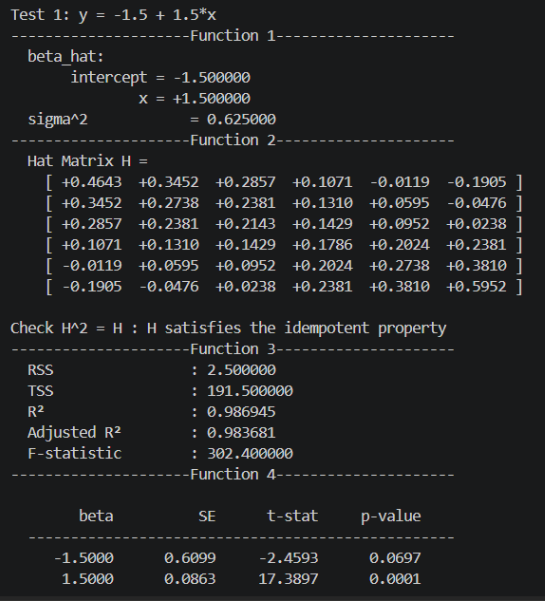
\includegraphics[width=0.85\textwidth]{images/part1/fig_test1_output.png}
    \caption{Kết quả Unit Test 1: $y = -1.5 + 1.5x$.
             Hàm \texttt{ols\_fit} cho $\hat{\beta}_0 = -1.5$, $\hat{\beta}_1 = 1.5$,
             $\hat{\sigma}^2 = 0.625$.}
    \label{fig:test1_output}
\end{figure}

\begin{figure}[H]
    \centering
    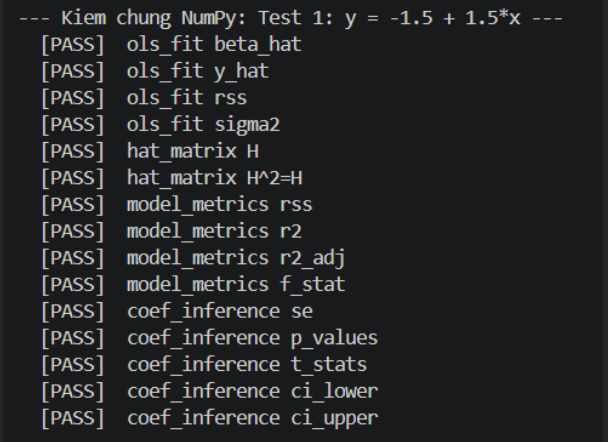
\includegraphics[width=0.75\textwidth]{images/part1/fig_test1_verify.png}
    \caption{Kiểm chứng NumPy -- Test 1: tất cả các mục đều \texttt{[PASS]}.}
    \label{fig:test1_verify}
\end{figure}

\begin{figure}[H]
    \centering
    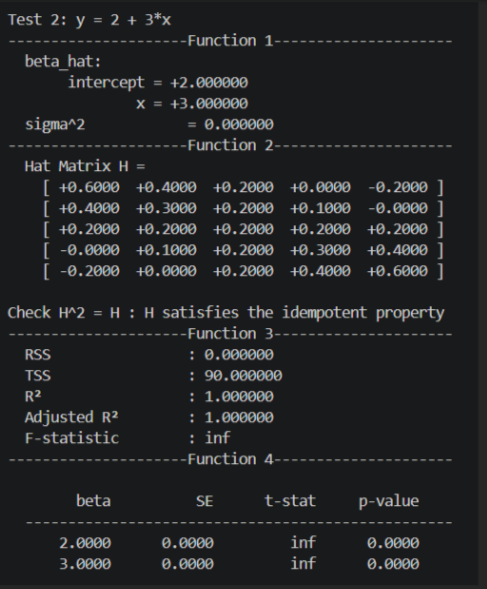
\includegraphics[width=0.85\textwidth]{images/part1/fig_test2_output.png}
    \caption{Kết quả Unit Test 2: $y = 2 + 3x$ (fit hoàn hảo, $\hat{\sigma}^2 = 0$,
             $R^2 = 1$, $F\text{-stat} = \infty$).}
    \label{fig:test2_output}
\end{figure}

\begin{figure}[H]
    \centering
    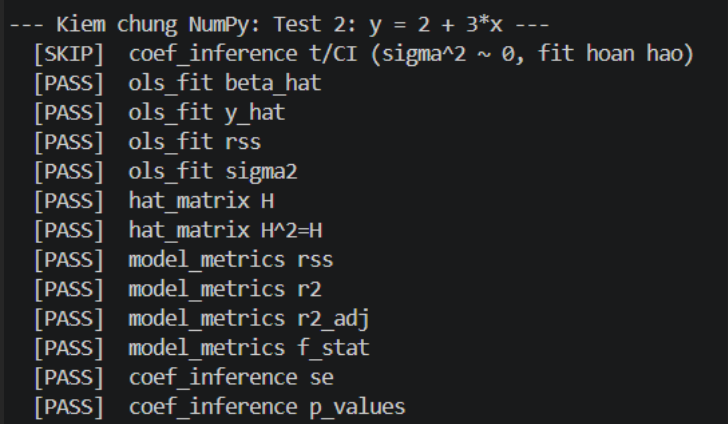
\includegraphics[width=0.75\textwidth]{images/part1/fig_test2_verify.png}
    \caption{Kiểm chứng NumPy -- Test 2: tất cả các mục \texttt{[PASS]}.}
    \label{fig:test2_verify}
\end{figure}

\begin{figure}[H]
    \centering
    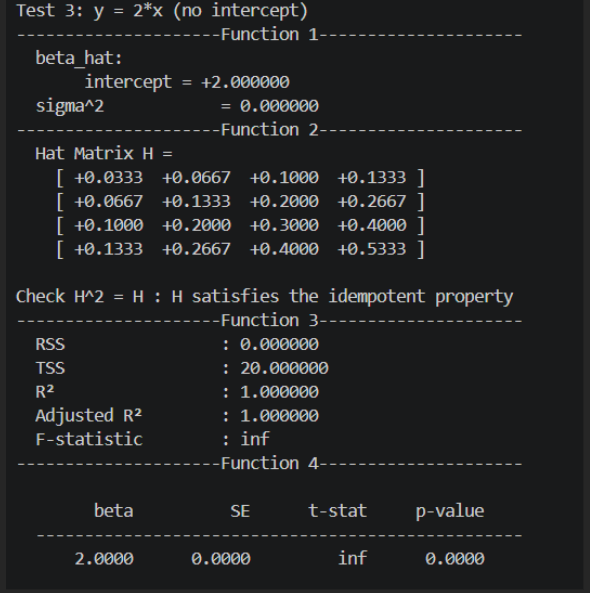
\includegraphics[width=0.85\textwidth]{images/part1/fig_test3_output.png}
    \caption{Kết quả Unit Test 3: $y = 2x$ (không intercept, fit hoàn hảo).}
    \label{fig:test3_output}
\end{figure}

\begin{figure}[H]
    \centering
    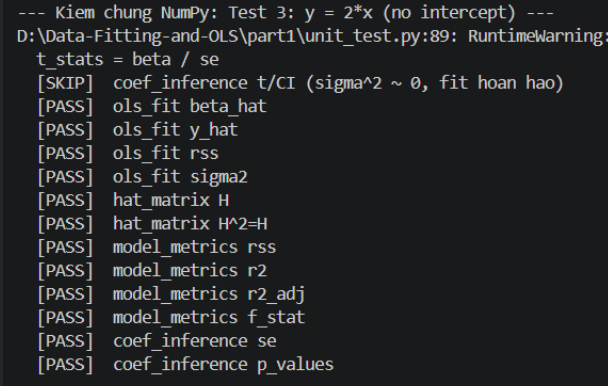
\includegraphics[width=0.75\textwidth]{images/part1/fig_test3_verify.png}
    \caption{Kiểm chứng NumPy -- Test 3.}
    \label{fig:test3_verify}
\end{figure}

\begin{figure}[H]
    \centering
    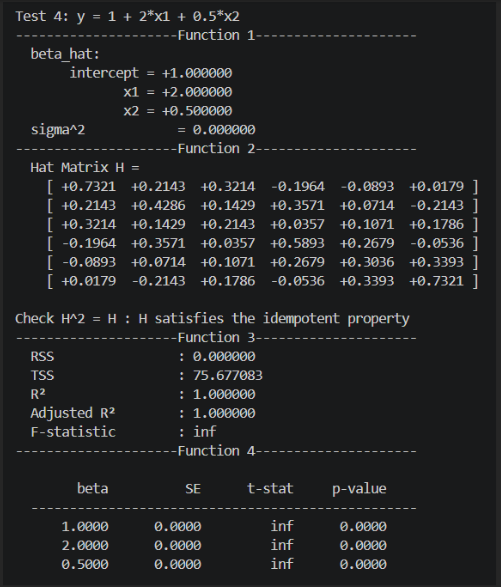
\includegraphics[width=0.85\textwidth]{images/part1/fig_test4_output.png}
    \caption{Kết quả Unit Test 4: $y = 1 + 2x_1 + 0.5x_2$.}
    \label{fig:test4_output}
\end{figure}

\begin{figure}[H]
    \centering
    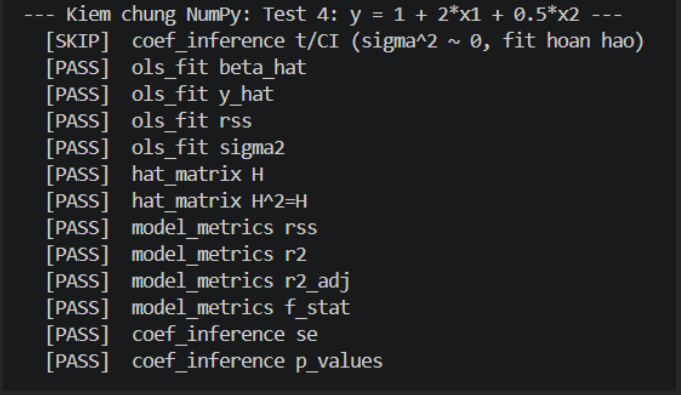
\includegraphics[width=0.75\textwidth]{images/part1/fig_test4_verify.png}
    \caption{Kiểm chứng NumPy -- Test 4.}
    \label{fig:test4_verify}
\end{figure}

\begin{figure}[H]
    \centering
    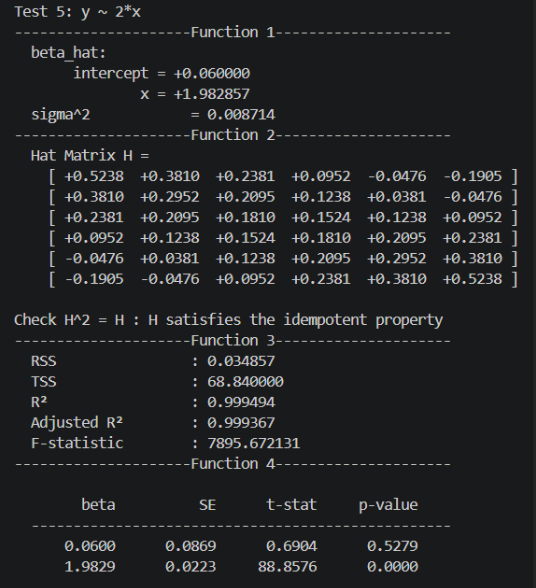
\includegraphics[width=0.85\textwidth]{images/part1/fig_test5_output.png}
    \caption{Kết quả Unit Test 5: $y \approx 2x$ (có nhiễu).
             $\hat{\beta}_0 \approx 0.06$, $\hat{\beta}_1 \approx 1.98$,
             $R^2 \approx 0.9995$.}
    \label{fig:test5_output}
\end{figure}

\begin{figure}[H]
    \centering
    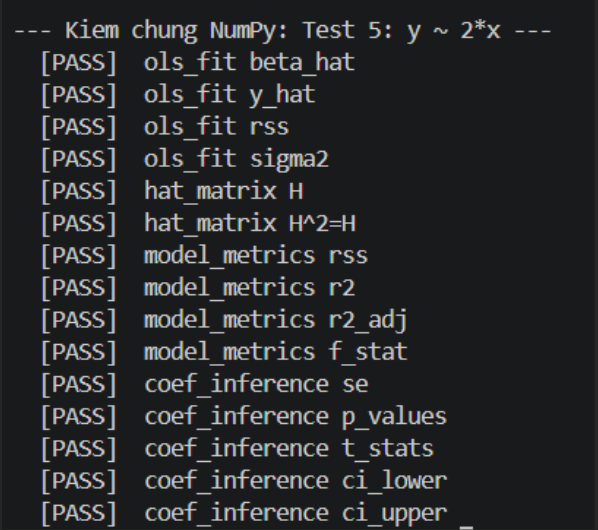
\includegraphics[width=0.75\textwidth]{images/part1/fig_test5_verify.png}
    \caption{Kiểm chứng NumPy -- Test 5: tất cả \texttt{[PASS]}.}
    \label{fig:test5_verify}
\end{figure}
\pagebreak
% ----------------------------------------------------------
\subsection{Hàm \texttt{hat\_matrix(X)}}

\subsubsection{Cơ sở Lý thuyết \& Công thức Toán học}

Hàm \texttt{hat\_matrix} tính ma trận mũ
$\mathbf{H} = \mathbf{X}(\mathbf{X}^\top\mathbf{X})^{-1}\mathbf{X}^\top$
và kiểm tra tính idempotent ($\mathbf{H}^2 = \mathbf{H}$) với ngưỡng sai số
$\mathrm{tol} = 10^{-8}$.
Hàm trả về dictionary: \texttt{H}, \texttt{is\_idempotent}, \texttt{n}, \texttt{k}.

Kết quả kiểm tra trên các unit test đã trình bày ở Yêu cầu 1 đều xác nhận
$\mathbf{H}^2 = \mathbf{H}$ và \texttt{[PASS] hat\_matrix H}, \texttt{[PASS] hat\_matrix H\textasciicircum2=H}.

% ----------------------------------------------------------
\subsection{Hàm \texttt{model\_metrics(y, \^{}y, p)}}

\subsubsection{Cơ sở Lý thuyết \& Công thức Toán học}

Hàm tính các chỉ số đánh giá mô hình: RSS, TSS, $R^2$, $\bar{R}^2$, và
$F$-statistic theo các công thức đã trình bày ở mục~\ref{}.
Hàm trả về dictionary: \texttt{rss}, \texttt{tss}, \texttt{r2}, \texttt{r2\_adj},
\texttt{f\_stat}, \texttt{df\_model}, \texttt{df\_resid}, \texttt{y\_mean}.

Kết quả kiểm chứng trên toàn bộ 5 unit test đều cho \texttt{[PASS]}.

% ----------------------------------------------------------
\subsection{Hàm \texttt{coef\_inference(X, y, \^{}β, σ²)}}

\subsubsection{Cơ sở Lý thuyết \& Công thức Toán học}

Hàm thực hiện kiểm định thống kê cho từng hệ số $\beta_j$:
\begin{enumerate}
    \item Sai số chuẩn: $\mathrm{SE}(\hat{\beta}_j) = \hat{\sigma}\sqrt{[(\mathbf{X}^\top\mathbf{X})^{-1}]_{jj}}$.
    \item $t$-statistic: $t_j = \hat{\beta}_j / \mathrm{SE}(\hat{\beta}_j)$.
    \item $p$-value (hai phía): $p_j = 2\,\mathbb{P}(T > |t_j|)$, $T \sim t_{n-p-1}$.
    \item Khoảng tin cậy 95\%: $\hat{\beta}_j \pm t_{0.025,\,n-p-1} \cdot \mathrm{SE}(\hat{\beta}_j)$.
\end{enumerate}
Hàm dùng phân phối $t$ cài đặt thủ công qua hàm beta không hoàn chỉnh chính quy
(\texttt{\_regularized\_incomplete\_beta}, \texttt{\_t\_cdf}, \texttt{\_t\_sf},
\texttt{\_t\_ppf}).

Kết quả kiểm chứng với SciPy cho \texttt{[PASS]} trên tất cả unit test có
$\hat{\sigma}^2 > 0$ (các test fit hoàn hảo được \texttt{[SKIP]} ở mục $t$/CI).

% ----------------------------------------------------------
\subsection{Hàm \texttt{vif(X)} -- Hệ số Phóng đại Phương sai}

\subsubsection{Cơ sở Lý thuyết \& Công thức Toán học}

Hệ số phóng đại phương sai (Variance Inflation Factor -- VIF) dùng để phát hiện và đo
lường mức độ nghiêm trọng của đa cộng tuyến trong mô hình hồi quy bội.
Công thức tính VIF cho biến $X_i$:
\begin{equation}
    \mathrm{VIF}_i = \frac{1}{1 - R_i^2},
\end{equation}
trong đó $R_i^2$ là hệ số xác định khi thực hiện hồi quy biến $X_i$ theo tất cả các biến
độc lập còn lại trong ma trận đặc trưng $\mathbf{X}$.
Quy tắc: VIF $\geq 5$ (hoặc $10$) là dấu hiệu đa cộng tuyến nghiêm trọng.

\subsubsection{Kết quả Cài đặt \& Kiểm chứng}

\begin{itemize}
    \item \textbf{Triển khai:} Thuật toán được cài đặt thủ công trong module
        \texttt{ols\_implementation.py} thông qua tính toán ma trận nghịch đảo để
        tìm $R_i^2$ cho từng biến.
    \item \textbf{Kiểm chứng:} Khởi tạo dữ liệu giả lập với 3 biến, trong đó
        $X_3$ có tương quan tuyến tính chặt chẽ với $X_1$ và $X_2$.
        Kết quả Unit Test cho thấy hàm tính chính xác VIF rất lớn cho $X_3$.
        Kết quả khớp hoàn toàn (sai số $\approx 0$) so với hàm
        \texttt{variance\_inflation\_factor} của thư viện \texttt{statsmodels}.
\end{itemize}

\begin{figure}[H]
    \centering
    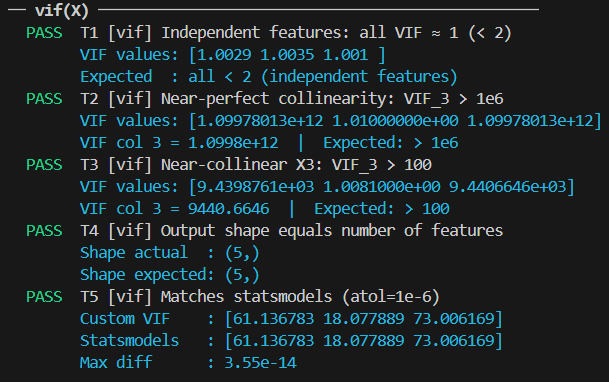
\includegraphics[width=0.85\textwidth]{images/part1/fig_vif_unittest.png}
    \caption{Unit test hàm \texttt{vif}: kết quả kiểm chứng so với \texttt{statsmodels}.}
    \label{fig:vif_unittest}
\end{figure}

% ----------------------------------------------------------
\subsection{Hồi quy Ridge -- Hàm \texttt{ridge\_fit(X, y, lam)}}

\subsubsection{Cơ sở Lý thuyết \& Công thức Toán học}

Khi xảy ra đa cộng tuyến, ma trận $\mathbf{X}^\top\mathbf{X}$ gần suy biến, khiến phương
sai của các ước lượng OLS bị thổi phồng. Hồi quy Ridge khắc phục điều này bằng cách thêm
đại lượng phạt $\lambda \geq 0$ vào đường chéo:
\begin{equation}
    \hat{\boldsymbol{\beta}}_{\mathrm{ridge}}
    = (\mathbf{X}^\top\mathbf{X} + \lambda\mathbf{I})^{-1}\mathbf{X}^\top\mathbf{y}.
\end{equation}
\textbf{Lưu ý:} Trong thực tiễn, intercept không bị phạt; phần tử $(0,0)$ của ma trận
phạt được gán bằng 0.

\subsubsection{Kết quả Cài đặt \& Kiểm chứng}

\begin{itemize}
    \item \textbf{Triển khai:} Hàm \texttt{ridge\_fit} được đóng gói trong module
        \texttt{ridge\_lasso.py}.
    \item \textbf{Kiểm chứng:} Kết quả vector hệ số khớp tuyệt đối với
        \texttt{sklearn.linear\_model.Ridge} (sai số $\approx 10^{-16}$).
    \item \textbf{Ridge Trace:} Đồ thị biểu diễn sự co rút (shrinkage) của các hệ số
        hồi quy khi $\lambda$ tăng dần -- các hệ số tiến về 0, giúp giảm độ phức tạp mô hình.
\end{itemize}

\begin{figure}[H]
    \centering
    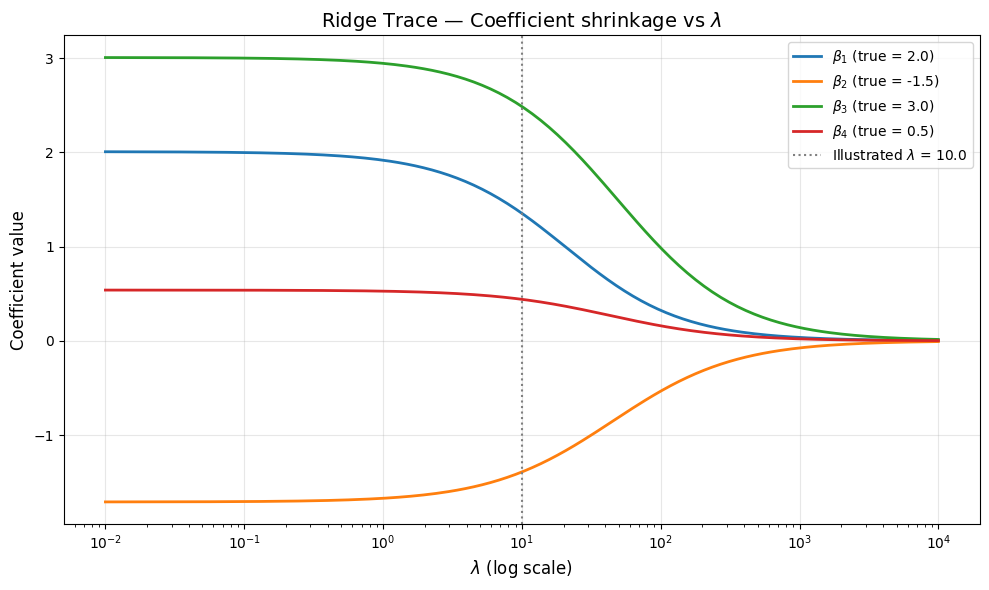
\includegraphics[width=0.85\textwidth]{images/part1/fig_ridge_trace.png}
    \caption{Đồ thị Ridge Trace: sự co rút của các hệ số hồi quy khi tăng mức phạt $\lambda$.}
    \label{fig:ridge_trace}
\end{figure}

\begin{figure}[H]
    \centering
    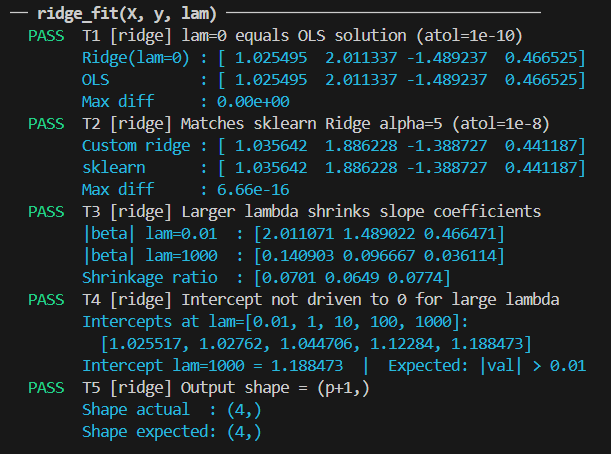
\includegraphics[width=0.85\textwidth]{images/part1/fig_ridge_unittest.png}
    \caption{Unit test hàm \texttt{ridge\_fit}: so sánh với \texttt{sklearn.linear\_model.Ridge}.}
    \label{fig:ridge_unittest}
\end{figure}
\pagebreak

% ----------------------------------------------------------
\subsection{Biểu đồ Phân tích Phần dư -- \texttt{residual\_plots}}

\subsubsection{Cơ sở Lý thuyết \& Công thức Toán học}

Để kiểm tra các giả định của hồi quy tuyến tính, ta sử dụng 4 biểu đồ chẩn đoán chuẩn
mực (theo định dạng \texttt{plot(lm())} trong R):

\begin{enumerate}
    \item \textbf{Residuals vs Fitted:} Kiểm tra tính tuyến tính và đồng phương sai.
        Lý tưởng: phần dư phân tán ngẫu nhiên quanh 0, không có xu hướng.
    \item \textbf{Normal Q-Q:} Kiểm tra phần dư có phân phối chuẩn.
        Lý tưởng: các điểm bám sát đường chéo.
    \item \textbf{Scale-Location:} Kiểm tra homoscedasticity (phương sai đồng đều).
        Lý tưởng: đường xu hướng phẳng.
    \item \textbf{Cook's Distance:} Xác định điểm ngoại lai ảnh hưởng mạnh.
        Công thức:
        \begin{equation}
            D_i = \frac{r_i^2}{p} \cdot \frac{h_{ii}}{1 - h_{ii}},
        \end{equation}
        với $h_{ii}$ là đường chéo của ma trận $\mathbf{H}$,
        $r_i$ là phần dư chuẩn hóa.
        Ngưỡng cảnh báo: $4/n$.
\end{enumerate}

\subsubsection{Kết quả Cài đặt \& Kiểm chứng}

\begin{itemize}
    \item \textbf{Triển khai:} Module \texttt{residual\_analysis.py} tự tính toán phần dư
        chuẩn hóa và ma trận Hat. Đồ thị Cook's Distance dạng bar chart với vạch ngưỡng
        $4/n$ tự động highlight và đánh số các điểm vượt ngưỡng.
    \item \textbf{Kiểm chứng:} Đồ thị Q-Q bám sát đường thẳng (phân phối chuẩn),
        phần dư phân tán ngẫu nhiên, các điểm ngoại lai được đánh dấu tự động.
\end{itemize}

\begin{figure}[H]
    \centering
    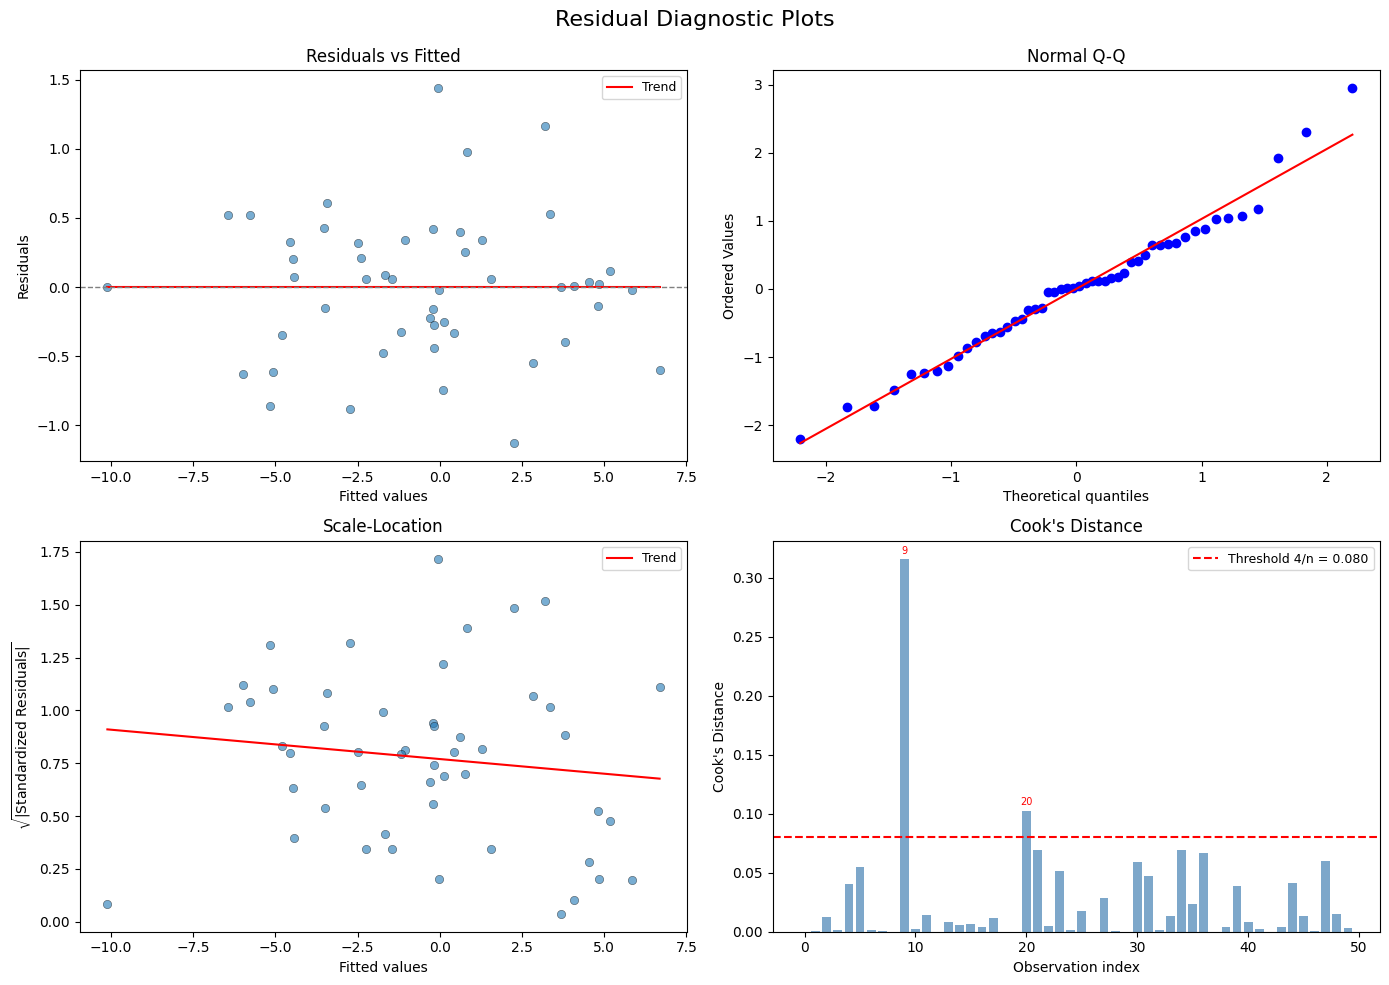
\includegraphics[width=\textwidth]{images/part1/fig_residual_plots.png}
    \caption{Bộ 4 biểu đồ chẩn đoán phần dư của mô hình OLS:
             Residuals vs Fitted, Normal Q-Q, Scale-Location, Cook's Distance.}
    \label{fig:residual_plots}
\end{figure}

\begin{figure}[H]
    \centering
    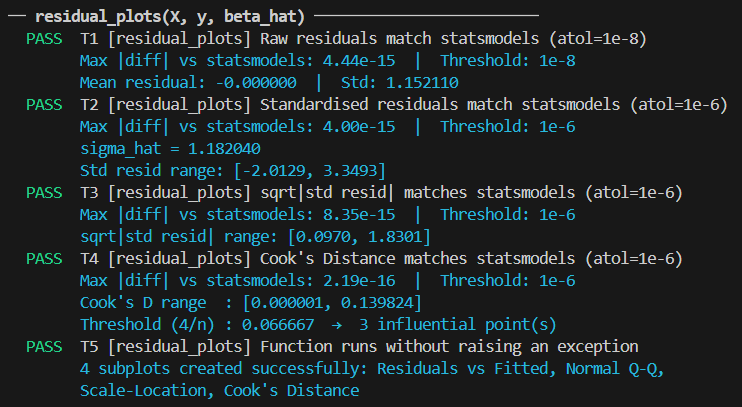
\includegraphics[width=0.85\textwidth]{images/part1/fig_residual_unittest.png}
    \caption{Unit test hàm \texttt{residual\_plots}.}
    \label{fig:residual_unittest}
\end{figure}

% ----------------------------------------------------------
\subsection{Kiểm định chéo K-Fold -- \texttt{kfold\_cv(X, y, k)}}

\subsubsection{Cơ sở Lý thuyết \& Công thức Toán học}

Phương pháp $k$-Fold CV ước lượng khả năng tổng quát hóa của mô hình một cách khách quan
hơn so với chia tập Train/Test đơn lẻ. Tập dữ liệu được chia đều thành $k$ phần ngẫu
nhiên. Vòng lặp $k$ lần lần lượt lấy 1 phần làm tập kiểm tra và $k-1$ phần làm tập huấn luyện.
Điểm đánh giá trung bình:
\begin{equation}
    \mathrm{CV}(k) = \frac{1}{k}\sum_{i=1}^{k}\mathrm{MSE}_i.
\end{equation}

\subsubsection{Kết quả Cài đặt \& Kiểm chứng}

\begin{itemize}
    \item \textbf{Triển khai:} Hàm \texttt{kfold\_cv} trong module
        \texttt{cross\_validation.py}, cố định \texttt{random\_state} qua
        \texttt{numpy.random.default\_rng(random\_state)} đảm bảo tính tái lập
        (reproducibility) hoàn hảo.
    \item \textbf{Kiểm chứng:} MSE trung bình và mảng MSE từng fold hoàn toàn trùng
        khớp với \texttt{cross\_val\_score} của \texttt{sklearn}. Với cùng tham số seed,
        kết quả chia fold giống nhau 100\%.
\end{itemize}

\begin{figure}[H]
    \centering
    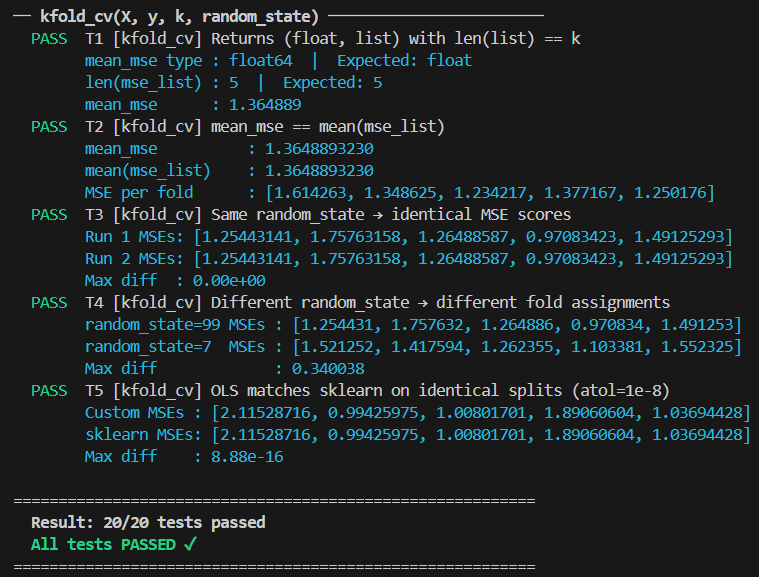
\includegraphics[width=0.85\textwidth]{images/part1/fig_kfold_unittest.png}
    \caption{Unit test hàm \texttt{kfold\_cv}: so sánh với \texttt{sklearn.cross\_val\_score}.}
    \label{fig:kfold_unittest}
\end{figure}

% ----------------------------------------------------------
\subsection{Minh họa Định lý Gauss--Markov (Monte Carlo)}

\subsubsection{Cơ sở Lý thuyết \& Công thức Toán học}

Theo định lý Gauss--Markov, trong số tất cả các ước lượng tuyến tính không chệch của
tham số $\boldsymbol{\beta}$, ước lượng OLS là tốt nhất (BLUE -- Best Linear Unbiased
Estimator) vì có phương sai nhỏ nhất:
\begin{itemize}
    \item \textbf{Không chệch (Unbiased):} $\mathbb{E}[\hat{\boldsymbol{\beta}}] = \boldsymbol{\beta}$.
    \item \textbf{Phương sai nhỏ nhất:}
        $\mathrm{Var}(\hat{\boldsymbol{\beta}}_{\mathrm{OLS}}) \leq \mathrm{Var}(\tilde{\boldsymbol{\beta}})$
        với mọi ước lượng tuyến tính không chệch $\tilde{\boldsymbol{\beta}}$ bất kỳ.
\end{itemize}

\subsubsection{Kết quả Cài đặt Mô phỏng (Monte Carlo)}

\textbf{Quy trình mô phỏng:}
\begin{enumerate}
    \item Thiết lập vòng lặp Monte Carlo $N = 2000$ lần.
    \item Mỗi lần lặp: sinh nhiễu ngẫu nhiên $\boldsymbol{\varepsilon}$, tính
        $\hat{\boldsymbol{\beta}}_{\mathrm{OLS}} = (\mathbf{X}^\top\mathbf{X})^{-1}\mathbf{X}^\top\mathbf{y}$.
    \item Đồng thời xây dựng \textbf{Ước lượng Tuyến tính Trọng số}
        $\hat{\boldsymbol{\beta}}_W = (\mathbf{W}^\top\mathbf{X})^{-1}\mathbf{W}^\top\mathbf{y}$
        với $\mathbf{W}$ là ma trận nhiễu. Cả hai đều tuyến tính và không chệch.
\end{enumerate}

\textbf{Kết luận mô phỏng:}
\begin{itemize}
    \item \textbf{Kiểm chứng không chệch:} Trung bình 2000 lần lặp của cả
        $\hat{\boldsymbol{\beta}}_{\mathrm{OLS}}$ và $\hat{\boldsymbol{\beta}}_W$ đều hội
        tụ rất sát về vector $\boldsymbol{\beta}$ thực tế.
    \item \textbf{Kiểm chứng phương sai (BLUE):} Phương sai của OLS luôn thấp hơn
        ước lượng trọng số. Trên đồ thị mật độ KDE, phân phối của OLS hẹp hơn,
        cao hơn, chứng tỏ OLS ít biến thiên và đáng tin cậy hơn.
\end{itemize}

\begin{figure}[H]
    \centering
    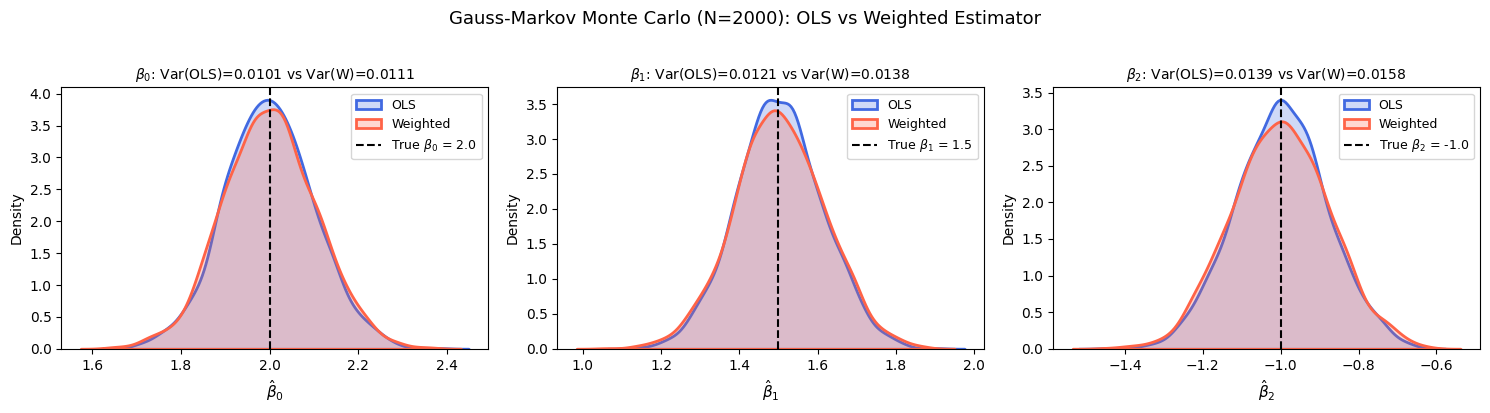
\includegraphics[width=\textwidth]{images/part1/fig_gauss_markov_kde.png}
    \caption{Biểu đồ mật độ phân phối (KDE) so sánh phương sai của OLS và ước lượng trọng số
             qua 2000 lần mô phỏng Monte Carlo.
             Phân phối OLS (đường hẹp, cao) cho thấy phương sai nhỏ hơn rõ rệt.}
    \label{fig:gauss_markov_kde}
\end{figure}

\begin{figure}[H]
    \centering
    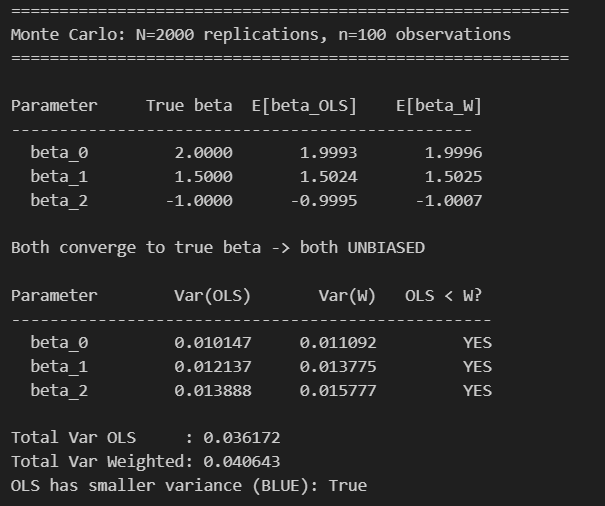
\includegraphics[width=0.85\textwidth]{images/part1/fig_gauss_markov_result.png}
    \caption{Kết quả chạy minh họa định lý Gauss--Markov bằng Monte Carlo:
             giá trị trung bình $\hat{\boldsymbol{\beta}}$ và so sánh phương sai.}
    \label{fig:gauss_markov_result}
\end{figure}
\pagebreak